\documentclass{beamer}
\usepackage{relsize}
\usepackage{color}

\usepackage{listings}
\usetheme{CambridgeUS}
%\usepackage{beamerthemesplit} % new 
\usepackage{enumitem}
\usepackage{amsmath}                    % See geometry.pdf to learn the layout options. 
\usepackage{amsthm}                   % See geometry.pdf to learn the layout options. There 
\usepackage{amssymb}                    % See geometry.pdf to learn the layout options. 
\usepackage[utf8]{inputenc} 
\usepackage{graphicx}
\usepackage[english,bulgarian]{babel}

\lstset{language=C++,
                basicstyle=\ttfamily,
                keywordstyle=\color{blue}\ttfamily,
                stringstyle=\color{red}\ttfamily,
                commentstyle=\color{green}\ttfamily,
                morecomment=[l][\color{magenta}]{\#}
}

\newtheorem{mydef}{Дефиниция}[section]
\newtheorem{lem}{Лема}[section]
\newtheorem{thm}{Твърдение}[section]

\DeclareMathOperator{\restrict}{\upharpoonright}

\setitemize{label=\usebeamerfont*{itemize item}%
  \usebeamercolor[fg]{itemize item}
  \usebeamertemplate{itemize item}}

\setbeamercovered{transparent}



\begin{document}
\title[Обектно ориентирано програмиране]{Сериализация} 
\author{Калин Георгиев} 
\frame{\titlepage} 

\section{Сериализация} 

\begin{frame}
\centerline{\texttt{f << data;}}
\centerline{\texttt{f >> data;}}
\end{frame}




\begin{frame}[fragile]
\frametitle{Първо изискване: обратимост}

\begin{flushleft}
\relscale{0.65}
\begin{lstlisting}
ostream& operator << (ostream& out, const DynArr<int>& ia)
{
  for (int i = 0; i < ia.size; i++)
    out << ia.arr[i];
  return out;
}
void test ()
{
  DynArr<int> arr (5);
  //...
  ofstream out ("data.txt");

  out << arr;
}
\end{lstlisting}  
\end{flushleft}

\begin{lstlisting}
[1,20,301,4,5] => 12030145
\end{lstlisting}  

\end{frame}


\begin{frame}[fragile]
\frametitle{Първо изискване: обратимост}

\begin{flushleft}
\relscale{0.65}
\begin{lstlisting}
ostream& operator << (ostream& out, const DynArr<int>& ia)
{
  for (int i = 0; i < ia.size; i++)
    out << ia.arr[i] << " ";
  return out;
}
void test ()
{
  DynArr<int> arr (5);
  //...
  ofstream out ("data.txt");

  out << arr;
}
\end{lstlisting}  
\end{flushleft}

\begin{lstlisting}
[1,20,301,4,5] => 1 20 301 4 5
\end{lstlisting}  

\end{frame}



\begin{frame}[fragile]
\frametitle{Второ изискване: еднозначност}

\begin{flushleft}
\relscale{0.65}
\begin{lstlisting}
ostream& operator << (ostream& out, const DynArr<int>& ia)
{
  for (int i = 0; i < ia.size; i++)
    out << ia.arr[i] << " ";
  return out;
}
void test ()
{
  DynArr<int> arr1 (5), arr2 (4);
  //...
  ofstream out ("data.txt");

  out << arr1 << arr2;
}
\end{lstlisting}  
\end{flushleft}

\begin{lstlisting}
[1,2,3]; [4,5,6,7] => 1 2 3 4 5 6 7
\end{lstlisting}  

\end{frame}


\begin{frame}[fragile]
\frametitle{Второ изискване: еднозначност}


\begin{flushleft}
\relscale{0.65}
\begin{lstlisting}
ostream& operator << (ostream& out, const DynArr<int>& ia)
{
  out << "[";
  for (int i = 0; i < ia.size-1; i++)
    out << ia.arr[i] << ",";
  if (ia.size > 0)
    out << ia.arr[ia.size-1];
  out << "]";
  return out;
}
void test ()
{
  DynArr<int> arr1 (5), arr2 (4);
  //...
  ofstream out ("data.txt");

  out << arr1 << arr2;
}
\end{lstlisting}  
\end{flushleft}

\begin{lstlisting}
[1,2,3]; [4,5,6,7] => [1,2,3][4,5,6,7]
\end{lstlisting}  

\end{frame}



\begin{frame}[fragile]
\frametitle{Оптимизация: предвидимост}

\begin{lstlisting}
[1,2,3]; [4,5,6,7] => [1,2,3][4,5,6,7]
\end{lstlisting}  

\begin{flushleft}
\relscale{0.63}
\begin{lstlisting}
istream& operator >> (istream& in, DynArr<int>& ia)
{
    DynArr<int> result(0); char c; int x;
    in >> c; assert (c == '[');
    while (c != ']' && in.peek() != ']')
    {
      in >> x;
      result += x;
      in >> c;
      assert(c == ',' || c == ']');
    }
    ia = result;
    return in;
}
void test ()
{
  DynArr<int> arr (0);
  ifstream in ("data.txt");
  in >> arr;
}
\end{lstlisting}  
\end{flushleft}


\end{frame}




\begin{frame}[fragile]
\frametitle{Оптимизация: предвидимост}


\begin{flushleft}
\relscale{0.65}
\begin{lstlisting}
ostream& operator << (ostream& out, const DynArr<int>& ia)
{
  out << ia.length() << " ";
  for (int i = 0; i < ia.size; i++)
    out << ia.arr[i] << " ";
  return out;
}
void test ()
{
  DynArr<int> arr1 (5), arr2 (4);
  //...
  ofstream out ("data.txt");

  out << arr1 << arr2;
}
\end{lstlisting}  
\end{flushleft}

\begin{lstlisting}
[1,2,3]; [4,5,6,7] => 3 1 2 3 4 4 5 6 7
\end{lstlisting}  

\end{frame}




\begin{frame}[fragile]
\frametitle{Оптимизация: предвидимост}

\begin{lstlisting}
[1,2,3]; [4,5,6,7] => 3 1 2 3 4 4 5 6 7
\end{lstlisting}  

\begin{flushleft}
\relscale{0.63}
\begin{lstlisting}
istream& operator >> (istream& in, DynArr<int>& ia)
{
    int newSize; in >> newSize; DynArr<int> result (newSize);
    for (int i = 0; i < newSize; i++)
    {
      in >> result[i];
    }
    ia = result;
    return in;
}
void test ()
{
  DynArr<int> arr (0);
  ifstream in ("data.txt");
  in >> arr;
}
\end{lstlisting}  
\end{flushleft}


\end{frame}


\begin{frame}
\centerline{Сериализация на хетерогенни контейнери}
\end{frame}



\begin{frame}[fragile]
\frametitle{``Записване'' на хетерогенен контейнер във файл}

\vspace{-60px}
\begin{center}
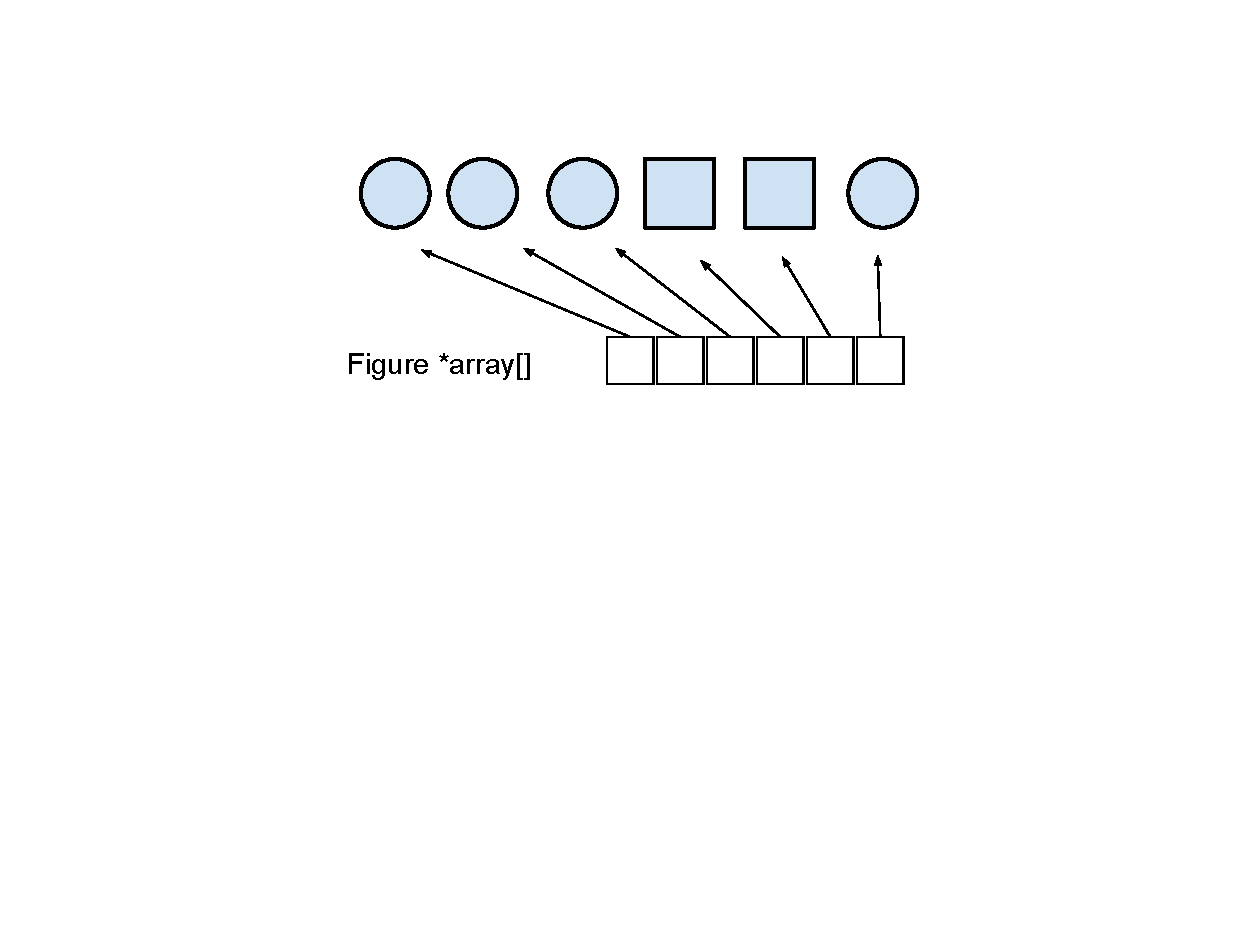
\includegraphics[width=12.0cm]{images/array}
\end{center}

\vspace{-160px}
\begin{lstlisting}
DynArr<Figure*> arr[10];
file << arr;
file >> arr;
\end{lstlisting}  

\end{frame}





\begin{frame}[fragile]
\frametitle{Директен подход не работи}

\begin{flushleft}
\relscale{0.63}
\begin{lstlisting}
ostream& operator << (ostream& out, DynArr<Figure*>& a)
{
  out << a.length() << " ";
  for (int i = 0; i < a.length(); i++)
    (1) out << a[i] << " ";     //Figure* ?!?!?
    (2) out << *a[i] << " ";    //Figure is abstract
    (3) out << a[i]->save(out);  //virtual function required
  return out;
}
void test ()
{
  DynArr<Figure*> arr[10]; //...
  ofstream out ("data.txt");
  out << arr;
}
\end{lstlisting}  
\end{flushleft}

\begin{itemize}
  \item Circle::save записва радиус
  \item Rectangle::save записва две страни
  \item save трябва да отговаря на всички условия за сериализиране
\end{itemize}

\end{frame}






\begin{frame}[fragile]
\frametitle{Трето изискване: Разпознаваемост}

\vspace{-60px}
\begin{center}
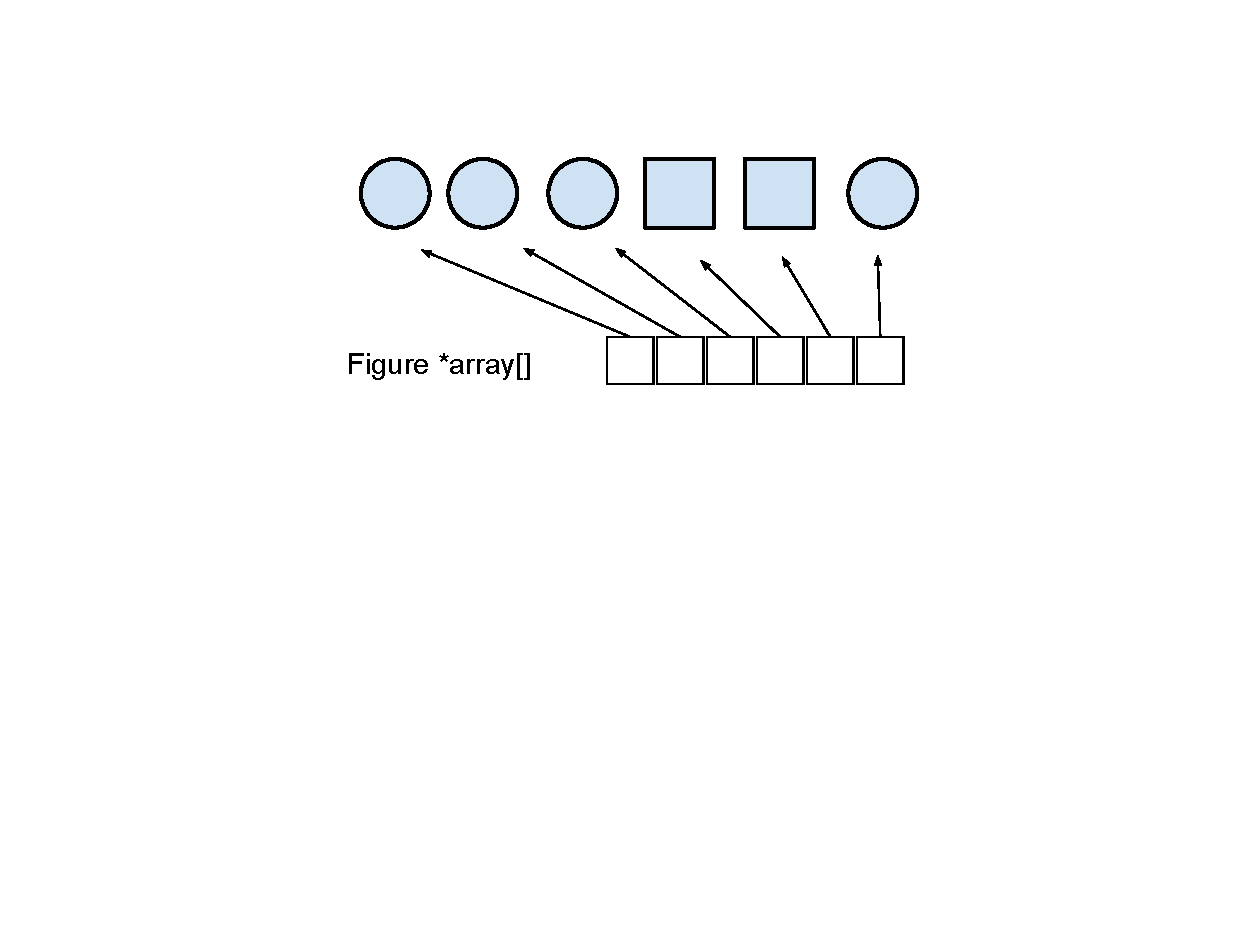
\includegraphics[width=7.0cm]{images/array}
\end{center}

\vspace{-80px}

\begin{itemize}
  \item Нека всички окръжности са с радиус 1, а всички правоъгълници със страни 2
\end{itemize}

\begin{lstlisting}
array => 6 1 1 1 2 2 2 2 1 
\end{lstlisting}  

\end{frame}

\begin{frame}[fragile]
\frametitle{Трето изискване: Разпознаваемост}

\vspace{-60px}
\begin{center}
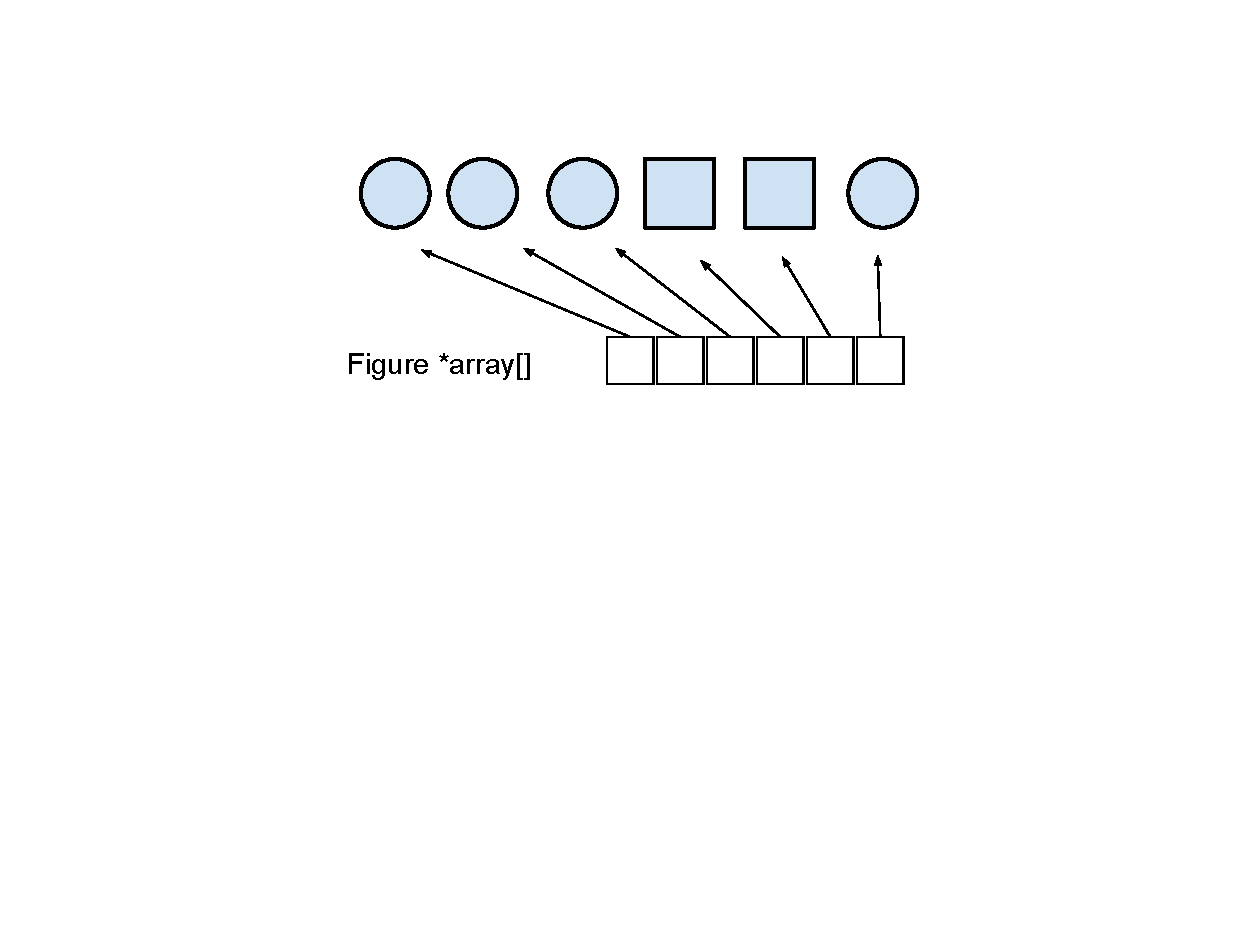
\includegraphics[width=7.0cm]{images/array}
\end{center}

\vspace{-80px}

\begin{itemize}
  \item Нека всички окръжности са с радиус 1, а всички правоъгълници със страни 2
\end{itemize}

\begin{lstlisting}
array => 6 1 1 1 2 2 2 2 1 
\end{lstlisting}  

\end{frame}



\begin{frame}[fragile]
\frametitle{Трето изискване: Разпознаваемост}

\begin{flushleft}
\relscale{0.73}
\begin{lstlisting}
void circle::save (ostream& out)
{ out << "circle " << r << " "; }
void rectangle::save (ostream& out)
{ out << "rect " << a << " " << b << " "; }
\end{lstlisting}  
\end{flushleft}

\begin{flushleft}
\relscale{0.73}
\begin{lstlisting}
array => 6 circle 1 circle 1 circle 1 rect 2 2 rect 2 2 circle 1 
\end{lstlisting}  
\end{flushleft}

\end{frame}



\begin{frame}[fragile]
\frametitle{``Фабрика'' за обекти}


\begin{flushleft}
\relscale{0.73}
\begin{lstlisting}
array => 6 circle 1 circle 1 circle 1 rect 2 2 rect 2 2 circle 1 
\end{lstlisting}  
\end{flushleft}

\begin{flushleft}
\relscale{0.73}
\begin{lstlisting}
istream& operator >> (istream &in, DynArr<Figure*> a)
{
  int newSize; in >> newSize; DynArr<Figure*> result (newSize);
  for (int i = 0; i < newSize; i++)
  {
    //what is result[i]???
    result[i]->read(in);
  }
}
\end{lstlisting}  
\end{flushleft}
\begin{itemize}
  \item read!
\end{itemize}

\end{frame}



\begin{frame}[fragile]
\frametitle{``Фабрика'' за обекти}


\begin{flushleft}
\relscale{0.73}
\begin{lstlisting}
array => 6 circle 1 circle 1 circle 1 rect 2 2 rect 2 2 circle 1 
\end{lstlisting}  
\end{flushleft}

\begin{flushleft}
\relscale{0.73}
\begin{lstlisting}
istream& operator >> (istream &in, DynArr<Figure*> a)
{
  int newSize; in >> newSize; DynArr<Figure*> result (newSize);
  for (int i = 0; i < newSize; i++)
  {
    result[i] = new WHAT; //WHAT?!?
    result[i]->read(in);
  }
}
\end{lstlisting}  
\end{flushleft}


\end{frame}







\begin{frame}[fragile]
\frametitle{``Фабрика'' за обекти}


\begin{flushleft}
\relscale{0.73}
\begin{lstlisting}
istream& operator >> (istream &in, DynArr<Figure*> a)
{
  int newSize; in >> newSize; DynArr<Figure*> result (newSize);
  string type;
  for (int i = 0; i < newSize; i++)
  {
    in >> type;
    result[i] = new type; //unfortunately NOT!!!
    result[i]->read(in);
  }
}
\end{lstlisting}  
\end{flushleft}



\end{frame}

\begin{frame}[fragile]
\frametitle{``Фабрика'' за обекти}


\begin{flushleft}
\relscale{0.73}
\begin{lstlisting}
istream& operator >> (istream &in, DynArr<Figure*> a)
{
  int newSize; in >> newSize; DynArr<Figure*> result (newSize);
  string type;
  for (int i = 0; i < newSize; i++)
  {
    in >> type;
    result[i] = new Figure::factory (type); 
    result[i]->read(in);
  }
}
\end{lstlisting}  
\end{flushleft}


\end{frame}



\begin{frame}[fragile]
\frametitle{``Фабрика'' за обекти}


\begin{flushleft}
\relscale{0.73}
\begin{lstlisting}
class Figure
{
  //....
  static Figure* factory (string type)
  {
    if (type == "circle") return new Circle (0);
    if (type == "rect") return new Rectangle (0,0);
    assert (false);
    return NULL;
  }
};
\end{lstlisting}  
\end{flushleft}


\end{frame}


\begin{frame}[fragile]
\frametitle{``Фабрика'' за обекти}


\begin{flushleft}
\relscale{0.73}
\begin{lstlisting}
class Figure
{
  //....
  virtual void read (istream &in) = 0;

  static Figure* factory (string type)
  {
    if (type == "circle") return new Circle (0);
    if (type == "rect") return new Rectangle (0,0);
    assert (false);
    return NULL;
  }
};
void Circle::read (istream &in)
{ in >> r; }
void Rectangle::read (istream &in)
{ in >> a >> b; }
\end{lstlisting}  
\end{flushleft}


\end{frame}





\begin{frame}[fragile]
\frametitle{``Фабрика'' за обекти}



\begin{columns}[t]
  \begin{column}{0.5\textwidth}
\begin{flushleft}
\relscale{0.5}
\begin{lstlisting}
istream& operator >> (istream &in, 
                      DynArr<Figure*> a)
{
  int newSize; 
  in >> newSize; 
  DynArr<Figure*> result (newSize);
  string type;
  for (int i = 0; i < newSize; i++)
  {
    in >> type;
    result[i] = new Figure::factory (type); 
    result[i]->read(in);
  }
}
\end{lstlisting}  
\end{flushleft}
  \end{column}
  \begin{column}{0.5\textwidth}
\begin{flushleft}
\relscale{0.55}
\begin{lstlisting}
class Figure
{
  //....
  virtual void read (istream &in) = 0;
  
  static Figure* factory (string type)
  {
    if (type == "circle") return new Circle (0);
    if (type == "rect") return new Rectangle (0,0);
    assert (false);
    return NULL;
  }
};
void Circle::read (istream &in)
{ in >> r; }
void Rectangle::read (istream &in)
{ in >> a >> b; }
\end{lstlisting}  
\end{flushleft}

  \end{column}
\end{columns}


\end{frame}


\begin{frame}
\centerline{Благодаря ви за вниманието!}
\end{frame}

\end{document}



\begin{columns}[t]
  \begin{column}{0.55\textwidth}

  \end{column}
  \begin{column}{0.45\textwidth}

  \end{column}
\end{columns}
